\documentclass[12pt]{article}
\usepackage[utf8]{inputenc}
\usepackage{svg}
\usepackage{hyperref}
\usepackage{listings}
\usepackage{xcolor}
\usepackage{booktabs} % For prettier tables
\usepackage{multicol}
\usepackage{multirow}
\usepackage[shortlabels]{enumitem}
\usepackage{hyperref}
\usepackage{cleveref}
\usepackage{subcaption}
\usepackage{fancyhdr}
\usepackage{outlines}
\usepackage{float}
\usepackage{array}
\usepackage{ragged2e}
\usepackage{multirow}
\usepackage{enumitem}
\usepackage{hyperref} 
\usepackage{pdfpages}
\usepackage{rotating}
\newcolumntype{P}[1]{>{\centering\arraybackslash}p{#1}} % center the column and justify its contents to the top in multirow tables
\newcolumntype{R}[1]{>{\RaggedLeft\arraybackslash}p{#1}} % Align column to the right in multirow tables

\definecolor{codegreen}{rgb}{0,0.6,0}
\definecolor{codegray}{rgb}{0.5,0.5,0.5}
\definecolor{codepurple}{rgb}{0.58,0,0.82}
\definecolor{backcolour}{rgb}{0.95,0.95,0.92}

\lstdefinestyle{mystyle}{
    backgroundcolor=\color{backcolour},   
    commentstyle=\color{codegreen},
    keywordstyle=\color{magenta},
    numberstyle=\tiny\color{codegray},
    stringstyle=\color{codepurple},
    basicstyle=\ttfamily\footnotesize,
    breakatwhitespace=false,         
    breaklines=true,                 
    captionpos=b,                    
    keepspaces=true,                 
    numbers=left,                    
    numbersep=5pt,                  
    showspaces=false,                
    showstringspaces=false,
    showtabs=false,                  
    tabsize=2
}

\lstset{style=mystyle}

% --- set footer and header ---
\renewcommand{\headrulewidth}{1pt}
\renewcommand{\footrulewidth}{1pt}
\title{Title}
\pagestyle{fancy}
\fancyhf{}

\makeatletter\let\Title\@title\makeatother

\lhead{\Title}
\rfoot{
\includegraphics[height=1cm]{Figures/logo_small.png}} % right header logo
\lfoot{
\includegraphics[height=1cm]{Figures/DocTide_logo.png}}
\setlength\headheight{16pt}
\setlength{\footskip}{50pt}
\lhead{\Title} %rightH title
\cfoot{\thepage}
% --- end footer and header ---

%----------EDIT COVER INFO HERE -----------------%

\def \LOGOPATH {Figures/ITU.svg}
\def \DEPARTEMENT {Department of Computer Science}
\def \COURSENUM {BIBAPRO1PE}
\def \COURSENAME {Bachelor Thesis}
\def \REPORTTITLE {Automating the Integration of LLM-Generated Software Documentation within GitHub Projects}
\def \STUDENTNAMEI {Markus Brandt Højgaard (mbrh@itu.dk)}
\def \STUDENTNAMEII {Lukas Brandt Pallesen (lupa@itu.dk)}
\def \INSTRUCTOR {Paolo Tell}

%------------------------------------------------%

%---------RESEARCH QUESTION-------------------
% \newcommand{\researchQuestion}{\textit{How can LLM-based agents be integrated into a GitHub Action to automatically generate sensible and non-intrusive code documentation, while maintaining the human in the loop?}}
% \newcommand{\researchQuestion}{\textit{How can a autonomous LLM-based agent be integrated into a GitHub Action to automate the task of making function level documentation, while maintaining the human in the loop?}}
\newcommand{\researchQuestion}{\textit{How can a autonomous LLM-based agent be integrated into a Github repository through Github Actions, to automate the task of generating method level documentation, \textcolor{red}{while maintaining the human in the loop?}}}
\newcommand{\subquestionI}{\textbf{What are the challenges when developing and integrating an autonomous agent into GitHub Actions?}}
\newcommand{\subquestionII}{\textbf{To what level is DocTide able to produce documentation comparable to that of a human developer?}}
\newcommand{\subquestionIII}{\textbf{How reliable is DocTide with regards to generating documentation in the correct format?}}

\begin{document}

\pagenumbering{Roman}

\begin{titlepage}
    \vfill
    \begin{center}
        \includesvg[width=0.7\textwidth]{\LOGOPATH} \\
        \hfill \\
        \Large{\DEPARTEMENT} \\
        \Large{\COURSENUM\;-\;\COURSENAME} \\
        \vfill
        \textbf{\LARGE{\REPORTTITLE}}
    \end{center}
    \vfill
    \begin{flushleft}
        \Large{\textbf{Prepared by:}} \\
        \Large{\STUDENTNAMEI} \\
        \Large{\STUDENTNAMEII} \\
        \Large{\textbf{Supervised by:} \INSTRUCTOR} \\
        \Large{\textbf{Date:} \today}
    \end{flushleft}
    \vfill
\end{titlepage}

%-----------------------------------------------%

%\tableofcontents
%\clearpage



\begin{abstract}
    This is a placeholder for an abstract. Before continuing, please, update your name, your supervisor's name, class code and the thesis title.

    Then follow the rest of the instructions and create and include custom sections.
\end{abstract}

\newpage

\tableofcontents

\newpage

\pagenumbering{arabic}
\fancyfoot[C]{Page \thepage\ of \pageref{EndOfText}}

%%%%%%% Note %%%%%%%
% The placeholder text is heavily influenced by the ACM proceedings template.
%%%%%%%%%%%%%%%%%%%%

\section{Introduction}
The notion of automation is not new in the realm of software development. As a part of the ever growing expectancy to the productivity in developing bigger and more complex system, the need for automation of processes in the software life-cycle was already seen as the necessary step to take back in 1985 where G. F. Hoffnagle and W. E. Beregi stated \textit{"Demand for reliable software systems is stressing software production capability, and automation is seen as a practical approach to increasing productivity and quality"}.
\\ \\
Similar to this it is well established that software documentation is a indispensable necessity in the \textit{software development life cycle}, acting as a constant vessel of quality. The area of the life cycle that benefits from documentation varies depending on the type of the documentation at hand, Aghajani et al.\cite{aghajani2020software} identifies source code documentation as of significant importance for especially \textit{software debugging} and \textit{program comprehension}.

However, to make documentation takes time, which developers often is in lack of, this introduces issues for the usefulness of documentation especial in regards to its '\textit{up-to-dateness}'\cite{aghajani2020software} where the survey conducted by Aghajani et al. shows that Missing documentations for a new feature/component, encounter Outdated/Obsolete reference and Code-documentation inconsistency is issues which is rated high in importance and is frequently encountered.
\\ \\
In software development Continuous Integration (CI) is a process which have been the place where test and build processes has been run in the effort to ensure a unified quality in the code base, serving as a automated guard towards introducing errors or bugs. When looking at systems to manage CI the landscape is varied, yet in a survey conducted by JetBrains on 26.000 developers, Github Actions comes out on top as the most used system by private developers, and the second overall.\footnote{https://www.jetbrains.com/lp/devecosystem-2023/team-tools/}
\\ \\
With the recent advancements of Large Language models (LLM), which have proven highly capable in creating natural language given specific context, the curiosity naturally arises on how such technological advancements could be used to mitigate some of the issues relates to current software documentation practices. Automatic documentation generation is researched as one possible mitigation, with Rai et al. identifying \textit{method level} source code documentation as an specific area of interest in contemporary research\cite{rai2022review}.
\\ \\
This paper contributes by investigating the possibility of extending the current CI practices with automatic generation of source code documentation. This is done by developing a prototype of an LLM-based autonomous agent under the restrictions of said agent running in Github Actions. A proposed framework for evaluating said agent in a environment simulating a live Github repository is propesed. Finally the implications on the design of the agent, brought by the Github Runner is discussed, and future directions is presented.

\subsection{Research question}
\researchQuestion
\section{Background}

\subsection{Software documentation}
Sommerville \cite{sommerville2001software} propose to generally sorting software documentation into two distinct classifications: \textbf{Process documentation} and \textbf{Product documentation}.
Where \textit{process documentation} enables management of the development of software, and includes types of documentation like plans, schedules or quality standards. \textit{Product documentation} covers describing the developed system, and can again be split into subcategories: \textit{user documentation} and \textit{system documentation}, the latter containing documentation embedded within code, generally referred to as \textit{source code documentation}.
\\\\
In their review of literature on the topic of automated software documentation, Rai et al. \cite{rai2022review} categorizes \textit{source code documentation} into three levels:
\begin{itemize}
    \item \textbf{Statement level:} Generally know as inline comments, used to explain small distinct pieces of the code.
    \item \textbf{Method level:} Covering informative naming, as well as summarization of methods or functions.
    \item \textbf{Class level:} Summarization of entire classes of code.
\end{itemize}

\subsection{Autonomous agent}
\label{sec:Autonomous agent}
The concept of \textit{ai agents} is gaining significant traction in the landscape of modern software development, with terminology such as \textit{agent}, \textit{autonomous agent} and \textit{ai agent} often used interchangeably. As shown in Fig. 3 of Wang et al.\cite{wang2024survey} the number of papers published in the field of LLM-based autonomous agents grew from near zero to beyond 160, between January 2021 to August 2023 alone.

A formal definition of the notion of \textit{autonomous agents} and how this differs from just ``normal" software, is proposed by Franklin et al. as follows:
\begin{quote}
    ``An \textbf{autonomous agent} is a system situated within and a part of an environment that senses that environment and acts on it, over time, in pursuit of its own agenda and so as to effect what it senses in the future."\cite{franklin1996agent}
\end{quote}

\subsection{Design of an autonomous agent}
\label{sec:BackgroundAgentDesign}
Wang et al.\cite{wang2024survey} proposes a unified framework for discussing LLM utilization in the design of an autonomous agent, by splitting the design into four \textit{`modules'}:
\begin{itemize}
    \item \textbf{Profile} module references the notion of influencing the LLM behavior of the agent through assigning a specific persona, role or personality. 
    \item \textbf{Memory} module looks at the agents ability to store, leverage and operate on the information collected from the environment, where it is proposed to differentiate between a \textit{unified} memory-structure modeling the capabilities of a the human short-term memory and a \textit{hybrid} memory-structure modeling both human short-term and long-term memory, as well as different \textit{memory-formats} the information can take. The \textit{memory operations} available to the module is how information from the environment is written into and read from its memory structure.
    \item \textbf{Planning} module is tasked with enabling the agent to emulate the human capability of breaking complex tasks into manageable steps, creating a plan for how to execute the task at hand. 
    \item \textbf{Action} module handles the translation of internal decisions of the agent into tangible outcomes. The collections of actions the agent can take is referred to as the \textit{action space}, and each action is described through its \textit{goal}, \textit{impact} and \textit{production}, where the latter describes how the action is executed.
\end{itemize}

\subsection{GitHub hosted runners}
\label{sec:githubRunner}
When executing a job in a GitHub Actions workflow, GitHub provides hosted virtual machine for the execution of said job; these are generally know as GitHub hosted runners (This paper will use the term GitHub runner). These runners is restricted to given specifications, depending on whether the repository is public or private. If we look at a Linux runner, the specifications is as follows:
\begin{itemize}
    \item \textbf{Public repository:} has a 4 CPU processor, 16GB RAM and 14GB SSD storage. The usage of runners on a public repository under these specifactions is free and unlimited.
    \item \textbf{Private repository:} has a 2 CPU processor, 7GB RAM, and 14GB SSD storage. The free usage of runners on a private repository is dependent on the given GitHub account.
\end{itemize}
\section{Related Work}
\subsection{Using LLMs to generate documentation}
\label{sec:related work LLM}
Research on LLMs ability to generate documentation from source code suggest that there is as potential for automating the task of documentation.
\\ \\
Khan and Uddin, \cite{10.1145/3551349.3559548} used a Chat GPT-3 based model called Codex, which is trained on natural language and code, to generate code documentations given source code from the CodeSearchNet dataset, covering six languages (Java, Python, PHP, Go, JavaScript, Ruby). Between the generated documentation and the original documentation from the dataset, several metrics was used to evaluated the result: BLEU score, to compare syntactic similarities, Documentation Length and Flesch-Kincaid Grade Level to compare the Quantity and Readability, TF-IDF score to compare informativeness, and a qualitative comparison by holding two examples up against each other. Showing that code documentation generated by Codex had satisfactory scores in the objective comparisons and even better understandability and extra information were added in the qualitative analysis.
\\ \\
Dvivedi et al. \cite{dvivedi2024comparativeanalysislargelanguage} conducted an analysis on how well LLM models generated code documentation given source code compared to the original code documentation. The model they used were, at the time, the most popular closed- and open-source LLM models, with sizes from 15 billion (Starchat) parameters to 1.76 trillion parameters. They looked at 5 objective metrics: Accuracy, Completeness, Relevance, Understandability and Readability. Concluding that \textit{"with the exception of Starchat, all LLMs demonstrated either equivalent or superior performance compared to the original documentation, highlighting their potential for automating documentation tasks"}.
\subsection{Autonomous Code Documentation Agents}
\label{sec: autonomus code documentaioin agents}
Looking at research on prototypes which tries to integrate code documentation generation to a repository, we see that the use of AI-driven Agents is the typical approach.
\\ \\
Yang et al.\cite{yang2025docagent} propose DocAgent, a multi-agent collaborative system, which generate documentation for a whole repository by leveraging the Chat GPT API. Working in two step: Firstly the Navigator makes a optimal process order, by examine the dependencies in the Repository. Secondly their multi agent system generates documentation for the whole repository.
\\ \\
Using the git pre-commit hook, Luo et al.\cite{luo2024repoagent} have made RepoAGENT which uses Chat GPTs API to created documentation files, which analyses the changes made in the commit, and updates the documentation files. This is an approach very similar to ours, by enabling of documentation in an CI pipeline system like GitHub Actions, provided you have an subscription to the Chat GPT API.
\\ \\
With confidence that various LLM is able to generate function level documentation, see \ref{sec:related work LLM}, this paper will contribute with a proposal to a autonomous code documentation agent prototype which will combine the two approaches mentioned above \ref{sec: autonomus code documentaioin agents} by both offer inline documentation and be integrated into a CI system to be able to keep documentation up to date. But also be in contrast by offering the agent as a free service without the need for a subscription to a cloud AI model, like Chat GPT API.


\newlist{qlist}{itemize}{1}
\setlist[qlist]{label=\textbf{Q1:}}
\newcommand\itemb{\item[\textbf{Q2:}]}
\newcommand\itemc{\item[\textbf{Q3:}]}

\section{Methodology}
\label{sec:method}
As stated in the introduction the contribution of this paper is to investigate the following:
\begin{quote}
    \researchQuestion
\end{quote}
The methodology used to do so, is to first identify the following three sub-questions, to clarify the challenges and limitations encountered by our approach and to evaluate on how well it works, to give an easy intuition on what this approach to autonomous code documentation agents offers, the sub-questions is as follows:

\begin{qlist}
    \item \subquestionI\textbf{:}
    Looking at what considerations one should take into account when designing an autonomous agent under the restrictions of integrating said agent into a github environment, and how challenges faced influences the proposed design.
    \itemb \subquestionII\textbf{:}
    The capabilities to generating function-level documentation of DocTide is compared to that of a human developer, since the intend behind developing DocTide as a LLM-based autonomous agent, is to automate the task of creating function-level documentation to a level comparable to that of a human developer.
    \itemc \subquestionIII\textbf{:}
    Since the core functionality of DocTide is to generate code which can be injected into the source code, and become function level source code documentation, it is necessary that both the syntax is correct such that the code can compile and that only documentation is created, and not executable code.
\end{qlist}


To investigate \textbf{Q1}, a prototype of an autonomous agent, DocTide is developed, following the design described in section \ref{sec:BackgroundAgentDesign}, to integrate into Github Actions. The results of this is presented in section \ref{sec:DesignDocTide}, and discussed in section \ref{sec:DiscussionQ1}. The types \textit{'human similarity metric'} and \textit{'success metric'} described in the \textit{LLM-based autonomous agent evaluation} section in Wang et al.\cite{wang2024survey} was identified as appropriate measures to address \textbf{Q2} and \textbf{Q3} respectively. These metrics are collected by running an experiment described in section \ref{sec:exp}, using a reusable evaluation framework, DocTide Labs (Section \ref{sec:DocTideLabs}). DocTide Labs was designed to facilitate the seamless integration of DocTide into a repository and to enable the systematic collection of data for the specified metrics.

The \textit{`human similarity metric'} is defined as the similarity in meaning between documentation DocTide creates and original documentation present in repository. This is scored using the CossEncoder from sentence transformers\footnote{\url{https://sbert.net/examples/cross_encoder/applications/README.html}} to get a semantic similarity score between existing function level documentation and function level documentation created be DocTide. To understand the scoring produced, the threshold is identified qualitatively between three buckets identified as follows:
\begin{itemize}
    \item \textbf{Low similarity:} Agent generated documentation fails to convey any of the information provided in the original documentation, or conveys wrong information.
    \item \textbf{Medium similarity:} Agent generated documentation convey some correct information reflecting parts of the original documentation, and no wrong information is provided.
    \item \textbf{High similarity:} Agent generated documentation correctly conveys the majority of information provided in the original documentation, only missing minute 
\end{itemize}
The results of this is presented in section \ref{sec:sem_results}, and discussed in section \ref{sec:DiscussionQ2}.

The core functionality of DocTide is to be able to inject function level documentation into source code, this has to be correctly formatted, otherwise malicious code, unintended or code braking behavior could be introduced. At a minimum, the documentation generated has to be of a valid comment type for the given programming language. Therefore the \textit{'success metric} is defined as the ratio between the number off successful formatted function level documentations generated by DocTide and the total number of attempted documentations. The results of this is presented in section \ref{sec:suc_results}, and discussed in section \ref{sec:DiscussionQ3}.

\subsection{AI usage disclaimer}
\textit{During the development of the code base for this project, openAI's ChatGPT 4o has been used as a tool for enhancing our software development. It has been used to understand the used frameworks and technologies as well as to understand error messages, but has not been used to generate code verbatim for the code base.
}
\section{DocTide}
\label{sec:DesignDocTide}
\subsection{Use case}
\textcolor{red}{example on Pull Request from DocTide }
DocTide works as an autonomous Agent by sensing changes to the repository via its integration as a GitHub Action, enabling developers to use it in there GitHub CI/CD pipeline, by adding the action to a workflow, as an example on how this could look like see \Cref{lst:flow}.
\begin{lstlisting}[language=Python, label={lst:flow}, caption=Example on how to use DocTide in a workflow]
jobs:
  DocTide_job:
    runs-on: ubuntu-latest
    name: Run Doctide
    steps:
      - name: Checkout
        uses: actions/checkout@v3
        with:
            fetch-depth: 0
      - name: DocTide Action
        uses: BrandtBoys/DocTide@v1
        with:
          testing: false
\end{lstlisting}
When the workflow is triggered, \Cref{fig:flow_doctide} shows how DocTide is run on a GitHub Runner with privilege to access the callers repository. Here DocTide finds the newly modified functions, added by the commit which triggered the DocTide workflow, and generates function level documentation for those functions. It commits the updated functions to an "update function level comments" branch and pushes it to the repository, creating a Pull Request for the developer of the code to accept or modify.
\begin{figure}[H]
\centering
\includegraphics[width=0.7\linewidth]{Figures/doctide_flow.png}
\caption{The use flow of DocTide}
\label{fig:flow_doctide}
\end{figure}
\subsection{Technical description}
As mentioned in section \ref{sec:method} the design of DocTide follows the proposed framework made by Wang et al. \cite{wang2024survey}, which has been explained in section \ref{sec:BackgroundAgentDesign}. This section will first present the technical components and dependencies which is used by DocTide, then this section will show how DocTide follows the design from Wang et al., to provide an understanding on how DocTide technically works as an autonomous agent.

The core functionality of DocTide comes from the python script doctide.py. As shown in \Cref{fig:components} doctide.py depends on external libraries, has some GitHub Action necessary configuration files and some extended functionality in a shared file with the test environment scripts, which in turn depends on other external libraries. This section will explain the components and how they relate to doctide.py.

\begin{figure}[H]
\centering
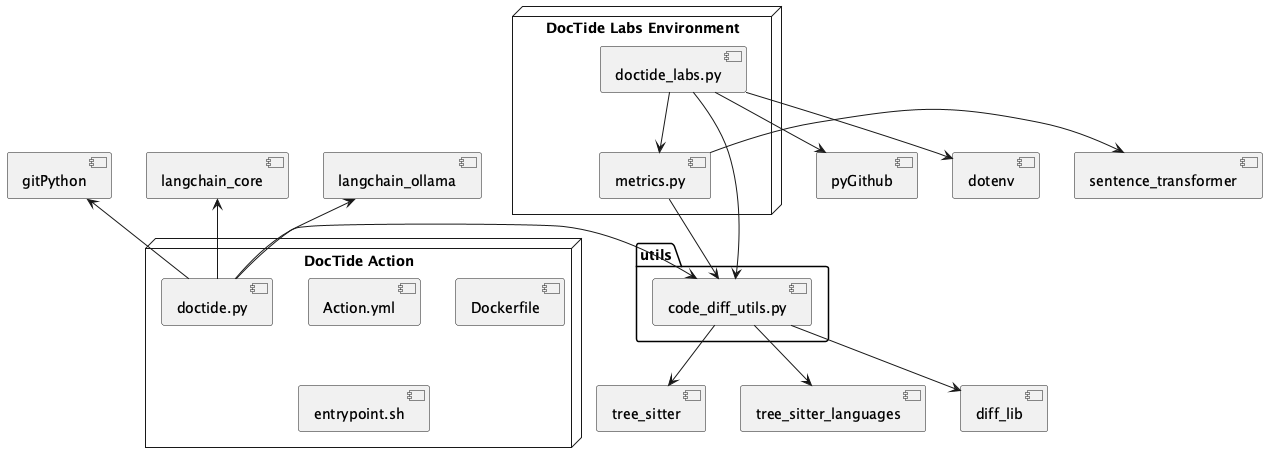
\includegraphics[width=0.7\linewidth]{Figures/component_diagram.png}
\caption{doctide.py dependencies and component structure}
\label{fig:components}
\end{figure}
\subsubsection*{gitPython}
GitPython\footnote{https://gitpython.readthedocs.io/en/stable/index.html} is used to have easy abstraction of git objects, enableing seamless interaction with a git repository. By passing the path to the working directory of the git repository of a system to the Repo("path") function, the system gets access to a pointer to the whole git repository. Which is easy in a GitHub Runner where the working directory is the equivalent to the working directory of the callers repository. It is now straight forward to create a branch and commit the generated function level documentations to that branch. And by creating a diff object between the most resent commit(HEAD) and second most resent commit (HEAD\(\sim \)1) using the Repo.head.commit and Commit.diff function, the most resent changes is identified which may call for generating and updating function-level documentation.
\subsubsection*{langchain}
Langchain is a framework for implement LLMs into a programming system. It is the core component in DocTide as it provides the local LLM which is used to generate the function-level documentation. DocTide uses the ollama service provided through \textbf{Langchain\_ollama.ChatOllama}\footnote{\url{https://python.langchain.com/api_reference/ollama/chat_models/langchain_ollama.chat_models.ChatOllama.html#langchain_ollama.chat_models.ChatOllama}}. Ollama is a vast library for LLMs which can be downloaded and run locally on a machine. Through the ChatOllama interface it is possible to specify which exact model from the Ollama library you wishes to use. To prompt the chosen model, the \textbf{langchain\_core.prompts.ChatPromptTemplate}\footnote{\url{https://python.langchain.com/api_reference/core/prompts/langchain_core.prompts.chat.ChatPromptTemplate.html#langchain_core.prompts.chat.ChatPromptTemplate}} offers a template to wrap the prompt for it to be in the right format for the ChatOllama.invoke function, which prompts the LLM with the given ChatPromptTmplate.
\subsubsection*{code\_diff\_utils.py}
Is a module created to seamlessly interact with the functionalities of tree-sitter (\ref{sec:tree-sitter}) and diff\_lib (\ref{sec:difflib}). Connecting tree-sitters ability to generate an abstract syntax tree (AST) for source code and diff\_libs ability to make diffs between two contexts, makes a reusable module for both doctide.py and doctide\_labs.py to avoid a lot of redundant code, and to have a framework which is easy to build new functionalities into, without having to build all the fundamentals again. This is done by the main function "extract\_data", which creates the AST of the source code, gain an understanding of which lines in the code has been modified and the traverses through the tree, and upon meeting a "function\_definition" node, it uses the handler function provided as an argument to do a specific task, which uses a helper function to identify a comment node. This ensures that the whole system follows the same logic on how the functions and function-level comments are identified, and is easy to modify and add functionalities by just making new handler functions.

\subsubsection*{tree-sitter}
\label{sec:tree-sitter}
To acquire contextual understanding of the modified files, an abstract syntax tree(AST) is created by passing the files with tree-sitter. An AST makes a tree like structure of the code, based on tokens which represents the building block of the code, so no matter what language the code was written in, the AST gives an abstract standardization of the code, which make it possible to processes files based on tokens instead of specific implementations. DocTide specifically uses the ASTs ability to identify function blocks and their associated comment style documentation. This also allows portability, in the future work of DocTide, since tree-sitter supports a large amount of programming languages, and can parse them into ASTs making it possible to analyze not only python but all the supported languages.

\subsubsection*{diff\_lib}
\label{sec:difflib}
Is a tool used to get the diff between the context of two versions of a file and therefor does not need a git reference to a commit to make a diff, which makes it quite flexible. To avoid a lot of redundant code between doctide.py and doctide\_labs.py in the analysis of the AST and which line were changed in the given two commits/contexts, the flexibility of diff\_lib was proven helpful as doctide.py and doctide\_labs.py uses two different tools to interact with git, gitPython and pyGitHub, which in terns also handles the way to look at diffs differently. But with diff\_lib, git is not relevant, and now both systems can use the code\_diff\_utils.py module

\subsection{Deployment as a GitHub Action}
To be able to integrate DocTide into a GitHub CI- pipeline, DocTide is deployed and accessible as a packaged Docker container action via the GitHub Marketplace, this section will go through how this is setup following the setup guide provided by GitHub \footnote{\url{https://docs.github.com/en/actions/sharing-automations/creating-actions/creating-a-docker-container-action}}. Public GitHub Actions are deployed to the GitHub Marketplace, wherefrom users are able to learn about the action and how to include it into there workflow. For DocTide to work as an action three files are necessary: Action.yml, Dockerfile and entrypoint.sh. 

\textbf{Action.yml} is a metadata file, which defines the setup for DocTide. It describes shortly what DocTide is and specifies its inputs and outputs and how it should be run. The latter is where it is specified that it uses docker to build an image of DocTide using the Dockerfile. 

The \textbf{Dockerfile} specifies the files DocTide consists of and where their source code is, such that it can be build into an image. 

Lastly the \textbf{entrypoint.sh} is the shell script which is run by the GitHub Runner (\Cref{sec:githubRunner}), this executes the login to GitHub via the Runners GitHub Token, installs the necessary python dependencies, installs Ollama and the chosen LLM, runs doctide.py and lastly commits generated function-level documentations to the callers branch. Which is what creates the pull request for the developers to modify or accept as is.
\subsubsection{Technical Design as an autonomous agent}
\textbf{Profiling}

DocTide has been given the specific role as a document assistance through the prompt given to the \textcolor{red}{LLM-model} as shown in \Cref{lst:prompt}

\begin{lstlisting}[language=Python, label={lst:prompt}, caption=Prompt used for the LLM]
    """
    You are a documentation assistant.

    ## Instructions:
    - Write a function-level documentation for the provided function, following best documentation practice for {program_language}
    Return **only** the comment

    ## Code:
    {code}
    """
\end{lstlisting}
\textbf{Memory}
\\
DocTide has a unified \textit{memory structure}, which means that information perceived from the environment only exist in local states inside the agent, and does not persist from run to run. The \textit{write operation} fetches the 'HEAD' commit and makes a diff with the 'HEAD\(\sim \)1'\footnote{The second latest commit on a repository} commit, identifying the latest changes to the repository. The \textit{memory format} of the diff is a structured list saved as diff\_files. The \textit{read operation} in DocTide is fairly simple as it just use the parameters \{program\_language\} and \{code\}, which is set by the planing module\ref{sec:planning module}, and read into the prompt.
\\ \\
\textbf{Planing and Action}
\label{sec:planning module}
The planing module is fairly simple, and does not rely on an LLM to plan the actions, but follows the sequence of the python script that is the backbone of the agent. \Cref{lst:plan_seq} shows as pseudo code the sequential order in which DocTide executes the actions following the the static plan. Given the simplistic nature DocTide as an autonomous agent, \ref{lst:plan_seq} also shows shows the entirety of the \textit{action space} for DocTide.

\begin{lstlisting}[language=Python, label={lst:plan_seq}, caption=The plan sequence of DocTides actions]
    - checkout_to_agent_branch
    for modified files:
        - detect_language
        - identify_modified_methods
            for modified methods:
            - generate_comment
            - validate_comment
    - commit_comments
    - write_to_testfile
\end{lstlisting}

\noindent
The \textit{production} of \textbf{write\_to\_testfile} is \textit{action via memory recollection}, as 
this action is triggered based on a 'testing' flag, read from the environment through memory. The remaining actions does all have \textit{action via plan following} as their production, meaning that they sequentially follow the plan. \textbf{detect\_language}, and \textbf{identify\_modified\_functions} has \textit{Environment Exploration} as their \textit{goal}, meaning the actions are aimed at deepening the agents understanding about its environment. The rest of the actions has \textit{Task Completion} as their \textit{goal}. The \textit{impact} of the actions is as followed:
\\\\
\textbf{checkout\_to\_agent\_branch:} is \textit{changing environment} of the agent, as the action serves to create a new branch for the agent to run on, and to checkout to this, effectively changing the state of the repository the agent is executing within.
\\ \\
\textbf{detect\_language:} extends the information know from the environment by detecting the language of the modified file, thus changing the \textit{internal state} of the agent.
\\ \\
\textbf{identify\_modified\_functions:} changes the \textit{internal state} of the agent by identifying which of the methods in the file has been modified in the latest commit.
\\ \\
\textbf{generate\_comment:} generates a method level comment for the modified method, adding this to the \textit{internal state} of the agent.
\\ \\
\textbf{validate\_comment:} handles validation of the generated method level comment, making sure that it follows the expected format and that it is not executable code. Based on the outcome of this validation, it then performs an \textit{action call} of the \textit{commit\_comments} action.
\\ \\
\textbf{commit\_comments:} handles add, commit and push of the newly generated method levels comments, thus \textit{changing the environment} of the agent.
\\ \\
\textbf{write\_to\_testfile:} if the agent is run with the 'testing' flag set to true, this action \textit{changes the environment} by handling writing test-data to a csv-file.

\subsection{Choice of LLM model}
The LLM which runs the code generation is the LLama 3.2 with 3 billion parameters. Its size is 2 gb which fits nicely to the hardware limits of the GitHub Runner (\Cref{sec:githubRunner})

\section{Evaluation framework - DocTide Labs}
\label{sec:DocTideLabs}
A long side the development of the LLM-based autonomous agent DocTide, this paper also proposes a framework, for conducting \textit{'objective evaluation'}\cite{wang2024survey} of said agents behavior and performance. Moving forward, this framework will be referred to as DocTide Labs.

DocTide Labs is an implementation of a \textit{'real world simulation protocol'}, in which the goal is to simulate an immersive environment where in the agent autonomously can complete tasks while chosen metrics\footnote{For the scope of this paper the only metrics collected are 'semantic similarity' and 'success rate', but the implemented evaluation protocol allows to be reused for collection of further metrics, if these where to be implemented.} are measured and collected\cite{wang2024survey}.
\\ \\
DocTide is developed as a prototype to automate the task of making function-level documentation within the environment of a Github repository, which is why DocTide Labs is developed to simulate exactly that. By replaying the commit history of a chosen Github repository and removing human generated documentation, DocTide Labs simulates the environment in which the agent is developed to run.

\subsection{Functionality\textcolor{red}{(Design?)} of DocTide Labs}
The logic and functionality of DocTide Labs is explained in the following sections. For a visualization of the entire flow of state when running an evaluation, see Figure \ref{fig:flow_labs}.
\\ \\
The only prerequisites to run DocTide Labs is a repository that you want to simulate in the evaluation, together with a Github Personal Access Token with `admin:org, gist, repo, workflow' permissions of said repository.

Furthermore before running, the part of the commit history to simulate during the evaluation is also specified.

\begin{figure}[H]
\centering
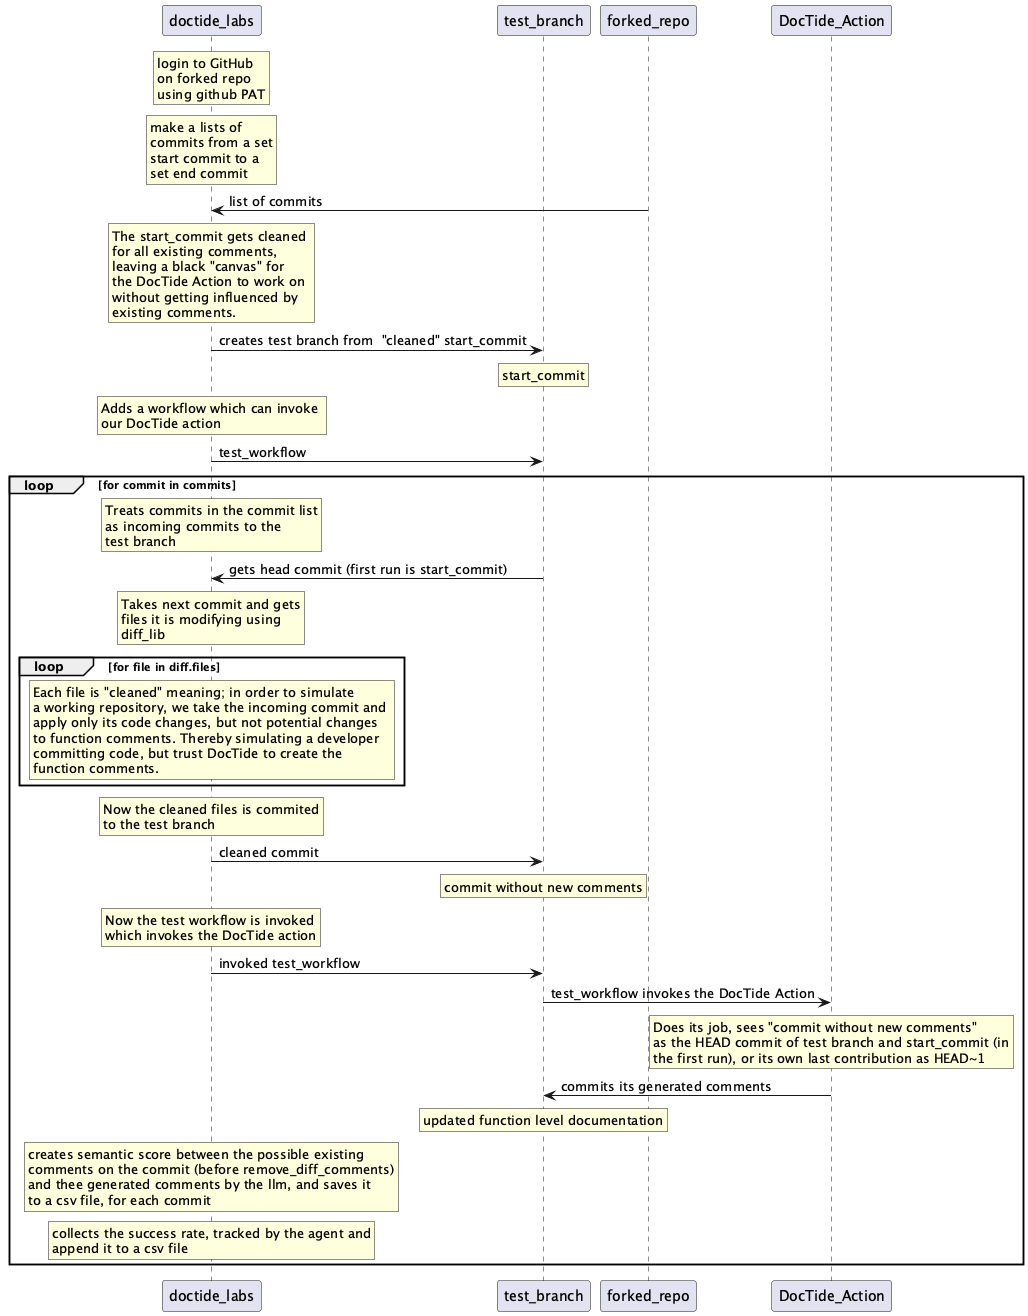
\includegraphics[width=0.7\linewidth]{Figures/doctide_labs_flow_chart.png}
\caption{The flow of the state the evaluation setup, shows how commits are collected from a repository, preprocessed, and then committed to the test-branch, where DocTide is invoked, and finally metrics are collected}
\label{fig:flow_labs}
\end{figure}

\subsubsection{Data Collection and setup}
The first step in DocTide Labs is to collect a 'dataset' of commits to use in the evaluation, which is done by fetching the specified commits from the chosen repository. All python files are cleaned from existing documentation, and a Test Branch is then created by checking out the oldest of the fetched commits, making this a 'snapshot copy' of the chosen repository in a previous time in history, but without the history of documenation.

Finally a workflow utilizing the DocTide Action is manually added to the repository, enabling DocTide Labs to trigger this later in the evaluation.

\subsubsection{Commit processing}
Next DocTide Labs then iterates through the fetched commits, processing each of them sequentially. In each iteration, first a diff between the commit and the head of the test branch is calculated, which serves to identify the files modified in the commit at hand. In order to best simulate the environment and conditions for which the agent is developed, each file in from the commit is then 'cleaned from comments'. This 'cleaning step' utilizes Tree-sitter\footnote{\url{https://tree-sitter.github.io/tree-sitter/}} to identify and remove all function-level documentation in the file, leaving only the code changes introduced with the commit. The diff of the cleaned file, and the head of the test branch is used to restore any documentation introduced by the agent in previous iterations.

Each 'cleaned commit' is then committed to the test branch, and the workflow utilizing the DocTide Action is triggered. This finalizes the simulation of the agent running continuously on a live repository that evolves over time.

\subsubsection{Agent execution and metric collection}
When triggered the workflow runs the agent, which generates the documentation based on the new commit. The Doctide Action is run with the 'testing' flag set to true, which allows it to directly merge in its generated documentation, enabling the continuous running of multiple iterations, without human intervention during the evaluation. 

Further more this enables the collection of metrics, which upon end of evaluation is returned in two csv files.

\section{Experiment}
\label{sec:exp}
To investigate \textbf{Q2} and \textbf{Q3} stated in \Cref{sec:method} an experiment is conducted, utilizing the evaluation framework DocTide Labs as described in section \ref{sec:DocTideLabs}. 
\\ \\
The evaluation is conducted using the opensource repository 'flask'\footnote{\url{https://github.com/pallets/flask}} as this is a well maintained opensource python repository, recognized for following a practice of method level documentation. 500 entries from the commit history ranging from \textit{'cabda59'} to \textit{'f61172b'} has been used as the commits to replicate during the evaluation.

As described in \cref{sec:method} two metrics is collected through this experiment: \textit{'semantic similarity} and \textit{'success rate'}

\subsection{Semantic Similarity}
Through the experiment when the DocTide agent generate documentation for a piece of code that has original documentation generated by a human developer, these pairs of documentation is collected. The Python module Sentence Transformers\footnote{\url{https://www.sbert.net/examples/cross_encoder/applications/README.html}} is then used to calculate the semantic similarity through running a Cross Encoder model.

Taking into considerations the efficiency of running this model over large quantities of comment pairs, we have decided to use the \textit{'stsb-roberta-base'} model, which scores 90.17 in the STSbenchmark\footnote{\url{https://sbert.net/docs/cross_encoder/pretrained_models.html}}.
\subsubsection{Identifying thresholds}
\label{sec:identifying thresholds}
Running the experiment resulted in the collection of \textbf{215} unique sets of documentation pairs and their semantic score, the distribution of which is seen in \cref{fig:sem_hist}.
\begin{figure}[H]
\centering
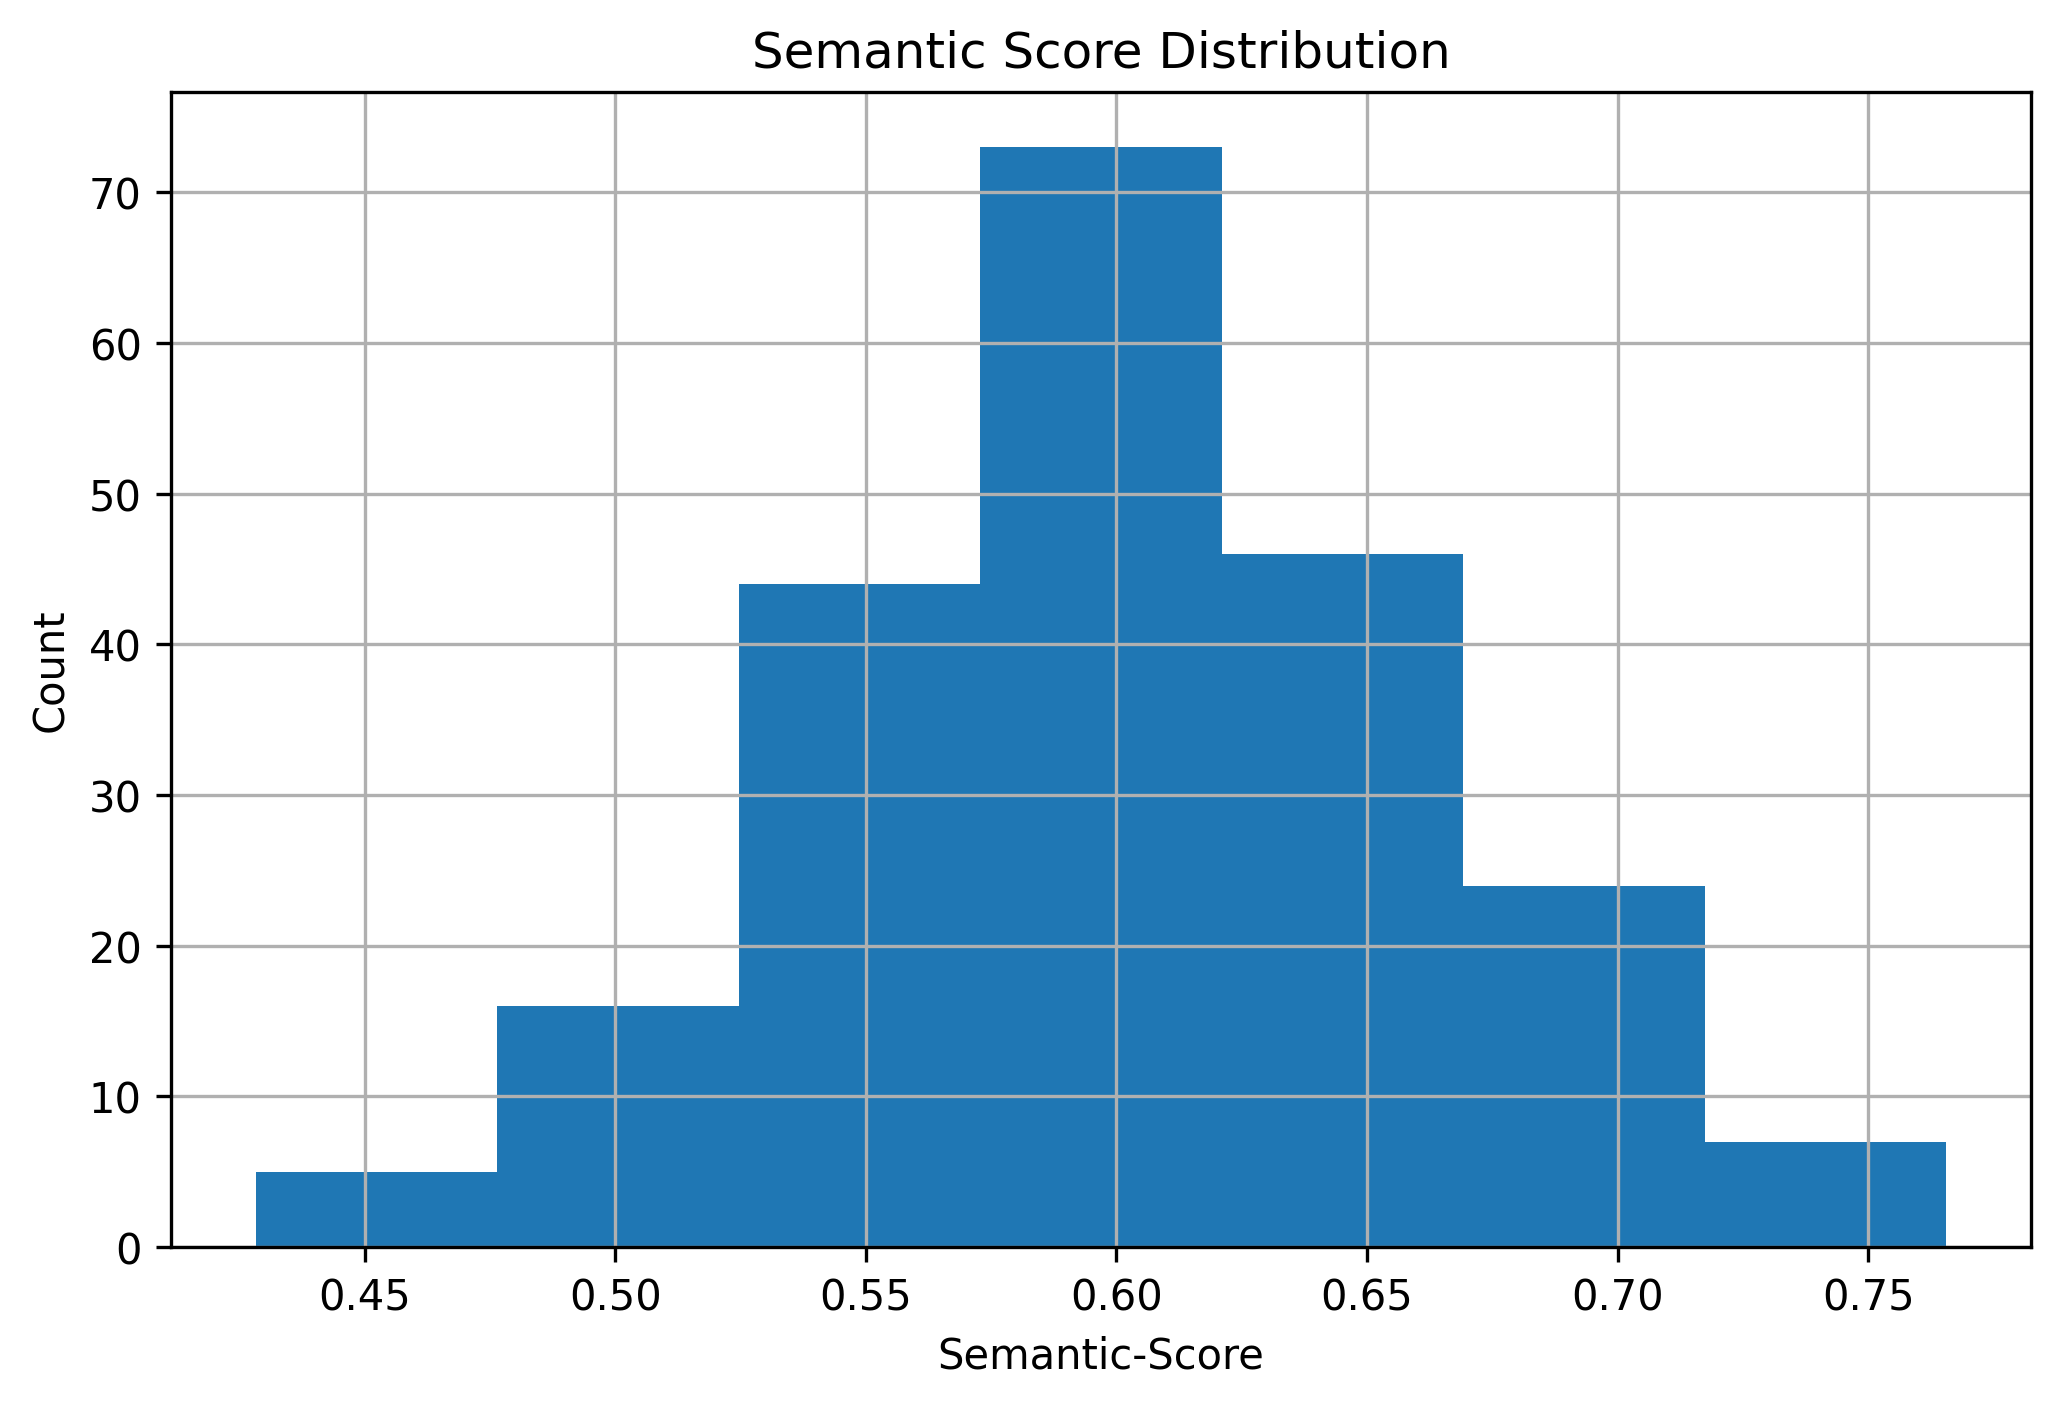
\includegraphics[width=0.7\linewidth]{Figures/semantic_score_histogram.png}
\caption{Histogram showing the normal distribution of the semantic-score metric collected}
\label{fig:sem_hist}
\end{figure}

Before being able to infer any information from this result, the result is processed in order to qualitatively identify the thresholds between the three quality buckets \textit{'Low-'}, \textit{'Medium-'} and \textit{'High similarity'} as described in section \cref{sec:method}.:
\\\\
First a \textbf{sample} is taken from the result pairs, which all contain the original documentation, the agent generated documenation and the semantic score. As seen in \cref{fig:sem_hist} the results follows a normal distribution, so the \textbf{sample} is taken to be representing of this, by utilizing \textit{stratified sampling}\footnote{\url{https://www.geeksforgeeks.org/stratified-sampling-in-pandas/}}. The column containing the semantic score is then hidden, and each pair is qualitatively inspected by comparing the original documentation to the agent generated documentation, before finally being assigned to one of the three quality buckets. For the entire results of this categorization of the sample, see table in \cref{appendix:sample_table}.

Next the \textbf{sample} is grouped by the assigned buckets, and summary statistics is calculated, before finally the thresholds is calculated as the midpoint between the maximum and minimum value of the higher and lower bucket respectively.:
\[
Low\_to\_medium = \frac{Max_{low}+Min_{medium}}{2} = 0.5590
\]
\[
Medium\_to\_high = \frac{Max_{medium}+Min_{high}}{2} = 0.6460
\]

\subsubsection{Results}
In \cref{fig:sem_box} the results of the experiment is plotted against the quality thresholds as identified in \cref{sec:method}, and from this it is shown that the majority of the data points falls within the buckets of \textit{medium-} and \textit{high similarity}, with the bucket of \textit{medium similarity} as the must frequent with more than 50\% of the data points.

\label{sec:sem_results}
\begin{figure}[H]
\centering
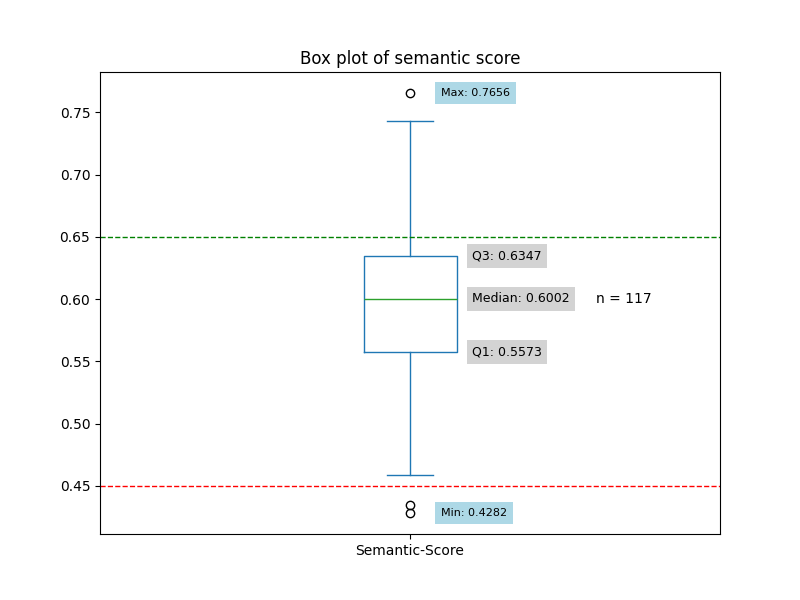
\includegraphics[width=0.7\linewidth]{Figures/semantic_score_box_plot.png}
\caption{Box plot visualizing the summary-statistics of the semantic scores against the identified thresholds.}
\label{fig:sem_box}
\end{figure}

\noindent
The exact distribution across the identified thresholds is as follows: 78.14\% of the results has a semantic score above the low threshold, and 22.79\% is above the high threshold, leaving 55.35\% to fall in the bucket of \textit{medium similarity} between the two thresholds.

\subsection{Reliability}
When running the DocTide agent with the 'testing' flag set to true, a success rate is collected for how many attempts ends with the agent generating documentation in the correct format.
Through the experiment, this is collected by a validation function \textit{validate\_response\_as\_comment()}, which is run for every response created. This function analyses the response from the LLM by creating a AST of the response using Tree-sitter\footnote{\url{https://tree-sitter.github.io/tree-sitter/}}, and then check that all nodes is of type comment.
We calculate the score by counting all successful formatted responses and all possible responses and then simply calculate the ratio between those two numbers.
\subsubsection{Reliability results}
\label{sec:suc_results}
Running the agent over the commits described for the experiment the DocTide agent attempted to generate documentation \textbf{945} times, out of which \textbf{652} were in the correct format. This means that 652 times the documentation generated by DocTide was able to re-integrate into the code base. This corresponds to a success\_rate of:
\[
Success\_rate=\frac{652}{945}*100\% = 68.99\%
\]

\subsection{Limitiations / Threats to validity}
The notion of success that we described in the method \Cref{sec:method} was build on knowledge obtained in the early stage of development, when we encountered that the LLM returned comments in markdown format, with the function definition at the beginning, with explanatory comments on what it has made, all formats which is not integrable into source code. Therefor we constructed this measurement of success based on the agents ability to generate documentation which would be integrable.
A potential thread to the internal validity is that it is the authors of the paper who made the qualitative comparison, when assessing which level of similarity there is between the two documentations. One could speculate if they were biased to try to make it follow the semantic score created by the Cross Encoder model, to make their results more significant and inferring a correlation between the semantic score and the qualitative similarity analysis. One of the limitation of the the level of intent DocTide is able to show is the level of build in intent in the function source code, since it does not have any other content then that. Some errors which were thrown under the execution of the testing framework has not been resolved like:
\begin{lstlisting}[language=bash, label={lst:unresolved_errors}, caption=Unresloved errors ]
    github.GithubException.UnknownObjectException: 404 {"message": "Not Found", "documentation_url": "https://docs.github.com/rest/repos/contents#get-repository-content", "status": "404"}
\end{lstlisting}

\textcolor{red}{Brainstorm: \begin{itemize}
    \item Thread to construct validity: Semantisk similarity sammenligner det med udvikler, det er godt da vi gerne vil immitere menneskelige evner for vores agent, men hvad hvis den originale documentation er dårlig? Måske tvilsomt, hvis vi bare holder os til at målet er at det skal have SAMME nivea som udviklere.
    \item Måske mere relevant er, vi får kun et datapunkt hvis der er original dokumentation. Hvad hvis de originale udviklere har været meget konservative med hvor de vil skrive dokumentation. Måske dette også åbner for snakken om at vi derfor siger at vi vil måle evnen til at 'generate dokumentation with same capabilities as a human developer", men vi måler ikke på den del af capabilities som er at vurdere hvor kode skal dokumenteres. Dette er noget vi ikke kan sige noget om baseret på vores data.
    \item Intent - Hvis ikke udviklere har været gode til at skrive intent ind i koden, så vil den aldrig kunne finde denne information, det kan føre til laverer scores.
\end{itemize}}
\section{Discussion}
In this section we will touch back on the stated sub-research-questions and discuss what value the applied method deliver when trying to answer these, and finally we discuss our initial research question and look at the bigger picture by looking at what initially motivated the paper and how this paper contributes in that regard.
\subsection{Q1 Discussion}
\label{sec:DiscussionQ1}
"\textit{\subquestionI}"
During development of DocTide several challenges and limitations was encountered in the quest to achieve the behavior of an autonomous agent on the hardware which the GitHub Runner provided. This section will discuss how these hardware limitation influenced the design of DocTide when trying to follow the proposed design of an LLM-based autonomous Agent from Wang et al.\cite{wang2024survey}.
\subsubsection*{Letting the LLM do it all}
The first approach was to find an LLM which fitted the hardware limitation, and as one of the first suggestions we met on Ollama was the llama 3.2 with a size of 2 gb in memory. Our intuition was that this size wouldn't exhorts the 14 gb RAM (\Cref{sec:githubRunner}), and therefor should be able to run fast. And when provided the whole file, on max 20 line, it did its job fairly good. But when we got our real world evaluation framework (\Cref{sec:DocTideLabs}) set up, it medially exposed the small LLMs limits when having to deal with file sizes of upwards to 600 lines (\Cref{appendix:A}). It is not possible to have a small LLM understand the whole context and write the whole file from scratch, hoping it have made sensible function level documentation, and not broken the code. 
\subsubsection*{Identifying the modified functions to document}
But since we had to stick with the small LLM, a way to offload the LLMs work, was to analyze the context on its behalf using tree-sitter and diff\_lib. If we should have stayed more true to the proposed agent design by Wang et al.\cite{wang2024survey} we should probably have tried to make a \textcolor{red}{LLM-drive planing module,|action?} which have identified and served the modified functions to an LLM-driven action which then could have generate the function level documentation. But since our level of trust in the small LLM to understand such large files had decreased, we opted for gaining more trust to the system by using static analysis. But this was not the only place we had to cut down the agents autonomy and using the content knowledge tree-sitter provides.
\subsubsection*{Write documentation back into the source code}
The test environment also exposed how the number of modified functions increased the actions execution time.
Execution times came upwards to 3 hours on merge commits, where multiply files was commit at once, and when investigating which process in the action that took so much time, and it was obvious that it was when the LLM had to write whole files and try to add the function level documentation the correct place. The approach with AST was further used to figure out where exactly a function level comment should be place given a specific modified function, relieving the LLMs task to only generate the function level documentation, provided the code of the modified function, and pass it to the insert functionality which takes the calculated byte offset to where the documentation should be, from the context of the AST, and insert it into the source code. The decreased the execution time significantly, but again we opted to go with an static analysis approach, rather than making a new LLM-based action which only purpose was to figure out where the most appropriate location for the documentation would be. The approach chosen gave us the most trust in that the agent would place the documentation at the right location, but we in turn decreased its autonomous abilities. And in fact, letting an LLM asses where it is appropriate to place a function-level documentation would make it more portable and not limited only identify where a comment should be placed given the supported programming language or level of documentation.
\subsubsection*{Ci integration}


\subsection{Q2 Discussion}
\label{sec:DiscussionQ2}
"\textit{\subquestionII}"
A semantic similarity score should, opposite to just looking at character comparison, give a quantitative measure for how much of the semantic meaning is present between two texts. This is why we chose to use the semantic similarity model from Sentence Transformers to compare the similarity between function-level documentation created by a human developer and by DocTide, to get a understanding of how similar to what the human developers intent to explain in a function-level documentation DocTide manages to generate. And in our qualitative analysis of the generated semantic similarity score(\Cref{sec:identifying thresholds}) we found this models scores to be a good indicate for this measurement. This measurement does not cover all attributes of documentation and does therefor not cover the all the ways to asses to what level DocTide is able to produce function-level documentation compared to that of a human developer, but it gives an indication on one of the more humane attributes by looking at what level DocTide captures the same intent with the documentation as the developer does.
Reflecting upon why the score was as it was, when looking at some of the data there were a correlation between poorly scored documentations and the developer documentation containing context which was derived from other files or how the function was used and not only its implementation. 
This could hypothesize that introducing more context to DocTide would improve its semantic scores, this hypothesis could be further motivated by having a developer create function-level documentation given only the source code of the function, operating under the same restrictions as DocTide, and see if the developers semantic score would follow the same distribution, indicating that it is the lack of context that is a factor for the level of similarity or if the developer scored higher, indicating that human intuition is a driving factor.
\subsection{Q3 Discussion}
\label{sec:DiscussionQ3}
"\textit{\subquestionIII}"
The results of the experiment as described in \cref{sec:suc_results} shows a \textit{'success\_rate'} for DocTide at \textit{68.99\%}, meaning that \textit{68.99\%} of the time the DocTide agent has attempted to generate documentation, it has resulted in documentation following the format described in \cref{sec:method} which has been inserted back into the code base. 
\subsubsection*{Current documentation coverage}
To discuss the implications of this, the python tool \textit{'docstr-coverage'}\footnote{\url{https://pypi.org/project/docstr-coverage/}} is ran on the same repository as the experiment was executed. This tool scans the entire codebase of the repository, identifies possible locations for method-level documentation, and meassures this coverage of these. As seen in \cref{lst:doc_percent_flask}, the results of this shows that the repository has method level documentation coverage of \textit{38.7\%}, implying that if the same project was ran with only DocTide handling documentation, the project would have a higher coverage of method level documentation than its current state. Though as found in \cref{sec:sem_results} not with the same level of information conveyed in each comment.

\begin{lstlisting}[language=sh, label={lst:doc_percent_flask},      caption= Ratio of method level documentation in flask repository]
    Needed: 8193  -  Found: 3169  -  Missing: 5024
    Total coverage: 38.7%  -  Grade: Not good
\end{lstlisting}

\subsubsection*{Format failures}
When looking at random samples collected from the 31.01\% of the dataset where the documentation generated does not follow the format described in \cref{sec:method}, two common reasons stands out as recurring reasons to format failure: the agent either misses the set of quotes actively 'closing' the comment, or the agent returns a copy of the method for which it is generating documentation as a prefix or suffix to the documentation itself. 

DocTide follows a very conservative approach where the attempt at generating documentation for a given function, is aborted when documentation not following the correct format is produced. After identifying the pattern of two common recurring reasons for format failure, it is hypothesized that integrating some form of internal feedback mechanism biased towards handling these exact cases could lead to an improvement in the 'success\_rate' metric. Similar to what is discussed in \cref{sec:DiscussionQ1}, this is limited by the capabilities of the LLM leading to a tradeoff between autonomy and trust.

\subsection{Overall discussion}
Following the design for LLM-based autonomous agents proposed by Wang et al.\cite{wang2024survey} has provided great direction and considerations on how to extend the autonomy of the agent and practical approaches to how to achieve that. However the development and integration of DocTide as a LLM-based autonomous agent has revealed a clear bias in our developing approach, which has shown evident in the solutions we resolved to when facing the challenges described in \Cref{sec:DiscussionQ1}. With a mindset of software developers working towards a working product, the limited size/capabilities of the LLM model the integration into GitHub Actions required, and the vitality of not injecting working code into the code base let to the identification of a notion of tradeoff between trust and autonomy. This notion was not something we found in research prior to the development of DocTide, but has show to be a beneficial cornerstone for the practical development of autonomous agents that aims to integrate into restriction of existing systems. For the development of DocTide, this resulted in the level of autonomy being scaled back to a minimum in order to ensure predictable behavior. This scale back and working with a more simple goal as we have done, with many of their concepts being derived from quiet complex systems, it have be challenging to keep a clear separation of the proposed modules when applying the theory into practice. Especial since their design relied on every module being driven by an LLM, and our prototype only using one instance of an LLM the lines became more blurred to the point where we decided to see the planing module and the action module as one, since it followed a sequential execution, and all actions followed the pre-defined plan. The level of trust in the capabilities of the LLM's utilized in the autonomous agent has shown to be what dictates the obtainable autonomy of the agent. As the field of LLM's and their capabilities currently is experiencing rapid evolution, it is therefore hypothesized that the boundaries and limitation of developing integrated autonomous agents capable of automating the task of making software documentation as well will be pushed. Why still choosing to follow this design proposal came to the potential that it offers, and how very few steps from the version DocTide is in now, will utilize the benefits of the structure.
\\\\
As stated in the \cref{sec:intro}, missing or outdated documentation as a result of developers lacking time is identified as an important issue that is frequently encountered. 

With 78.14\% of the documentation generated by DocTide achieving \textit{medium-} and \textit{high similarity} to documentation produced by human developers, and a \textit{'success rate'} of 68.99\% on generating and reintegrating documentation in the correct format, DocTide as a prototype manages to support the claim that an integrated autonomous agent would be able to mitigate the severity of the missing or outdated documentation. The direct integration into GitHub actions enables these benefits without the need of human interference, changing the state of documentation from opt-in to opt-out.

\subsection{Future work}
We will here describe which next step for DocTide we would be interested to investigate:
\subsubsection*{Gaining more context}
As mentioned in \Cref{sec:DiscussionQ2}, increasing DocTides context of the source code and the context in which the code is would maybe be a factor to increasing its level of similarity. This could simply be done in giving it the code of the whole file in which the function is situated in, or make an dependency analysis to give give more knowledge of the surrounding context.
\subsubsection*{Let the agent validate its response}
As discussed in \cref{sec:DiscussionQ3} it is hypothesized that implementing a feedback mechanism to enable re-attempting the generation of documentation after failing on format in the first attempt, could lead to an increase in the \textit{'succes rate'} of the 

Following \cite{wang2024survey} one consideration could be to implement \textit{model feedback} where internally an LLM is used instead of DocTides static format check, to decide whether the generated documentation follows correct format and to handling \textit{re-prompting} in the case that it does not.

\subsubsection*{Enable DocTide to evolve based on feedback from Pull Requests}
As developers will be prompted with a pull request, containing DocTides generated function level documentation, they will either accept it, modify it or reject it. A future work could be to find a way to harvest this valuable feedback, to enable DocTide to learn and evolve by saving its learning to a persistent memory structure.
\section{Conclusion}
\researchQuestion
\begin{itemize}
    \item
\end{itemize}
\label{EndOfText}

\newpage
\pagenumbering{Roman}
\fancyfoot[C]{Page \thepage\ of \pageref{endOfDoc}}
\bibliographystyle{IEEEtran}
\bibliography{IEEEabrv,cites}

\newpage
\appendix
\section{Naive approach, handling a large file poorly}
\label{appendix:A}
\includepdf[pages=30]{appendix/Naive-agent-commit-to-flask.pdf}

\section{Sample for semantic similarity data processing}
\label{appendix:sample_table}
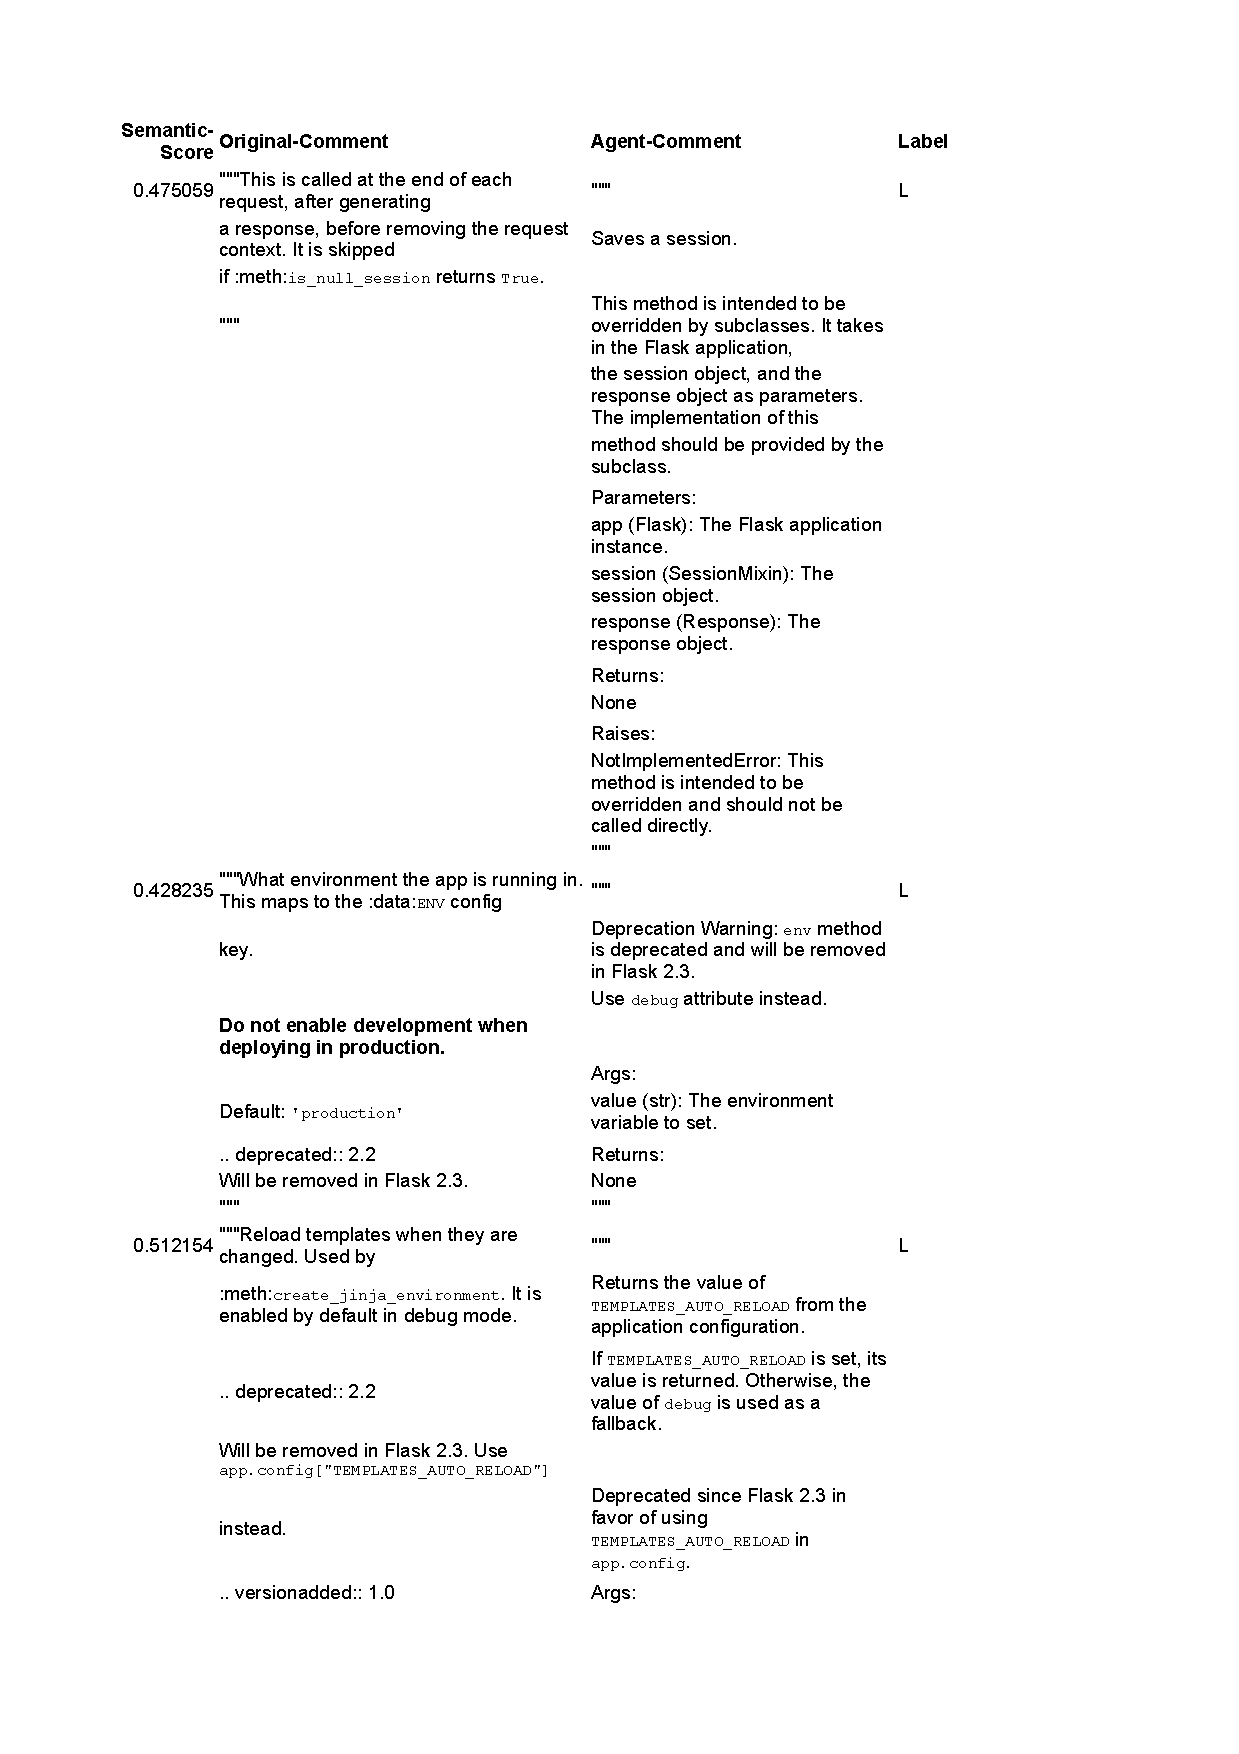
\includepdf[pages=-]{appendix/semantic_sample.pdf}
\label{endOfDoc}

%\clearpage

%\listoffigures

%\clearpage

%\listoftables

%\clearpage

%\listoflistings

\end{document}